\begin{frame}[fragile]
  {\Huge Kernels update}

  \begin{itemize}
  \item Architectures support
  \item Batched linear solvers
  \item Block Sparse Matrices
  \item Batched GEMM
  \item Mixed precision
  \end{itemize}

\end{frame}

\begin{frame}[fragile]{Platforms/Architecture support (Brian, Luc)}
Architecture support:
\begin{itemize}
  \item Nvidia fully supported with Cuda backend
  \item AMD fully supported with HIP backend, still optimizing for performance
  \item Intel initial support with SYCL backend, more testing and performance optimization needed
\end{itemize}
Spack updated with release 3.6.0, build tested on Summit, Spock/Crusher and initial support on Arcticus.\\
Starting to support streams on device, inquire for details.
\end{frame}

\begin{frame}[fragile]{Batched Linear Solvers (Kim)}
New batched linear solvers are introduced
\begin{itemize}
  \item LU with static pivoting
  \item PCG
  \item GMRES
\end{itemize}
\begin{center}
  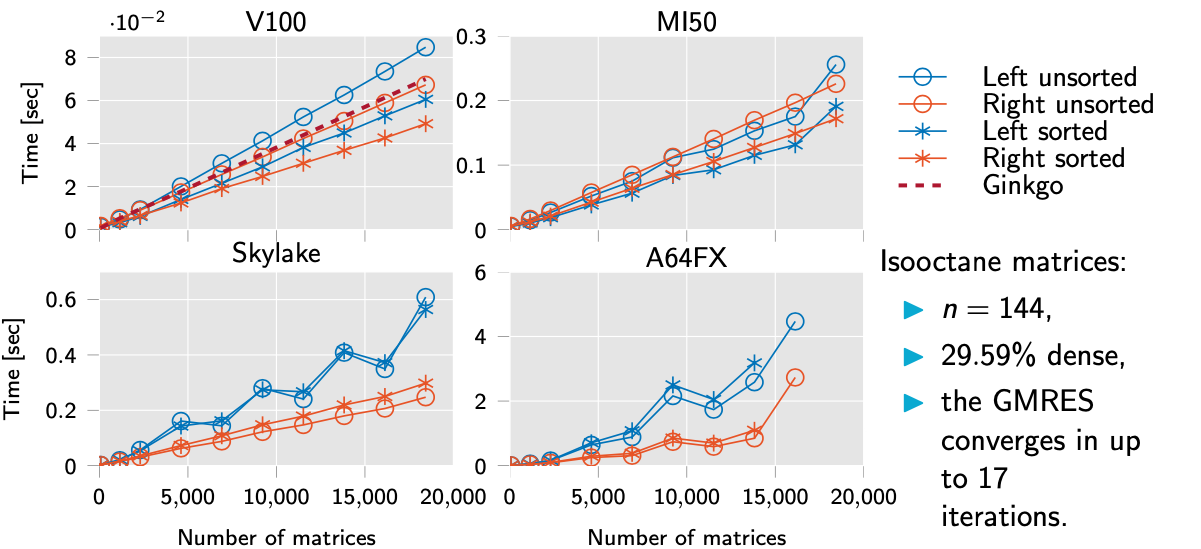
\includegraphics[scale=0.2]{batchedGMRES}
\end{center}
\end{frame}

\begin{frame}[fragile]{Block Sparse Matrices: BsrMatrix (NGA, Luc)}

New BsrMatrix matrix format implemented, supports constant block size sparse matrix mostly geared toward multi-physics systems representation.\\
Currently supported algorithms:
\begin{itemize}
  \item BrsMatrix
  \item Matrix-Vector product using SpMV interface
  \item Matrix-Matrix product using SpGEMM interface
  \item Gauss-Seidel smoother
\end{itemize}
The new format requires less memory and exposes dense linear algebra usage within sparse linear algebra kernels, leading to increased performance compared to point CrsMatrix.

\end{frame}

\begin{frame}[fragile]{Batched GEMM improvements (Evan, Vinh)}
New heuristics and improved interface included a unified interface for all levels of parallelism (TeamVector, Team and Serial) for simplicity.\vspace{-1em}
\begin{columns}[t,onlytextwidth]
  \column{.6\textwidth}
  \begin{itemize}
  \item row-major speedup is 1.17x
  \item column-major speedup is 1.26x
  \item dimensions 2 to 24: single parallel-for with a RangePolicy over entries of C
  \item dimensions $>$ 24: double buffering algorithm based on Magma’s BatchedGemm, Kokkos team cooperatively works on a tile.
  \end{itemize}
  \column{.05\textwidth}
  \column{.35\textwidth}
  \begin{figure}
    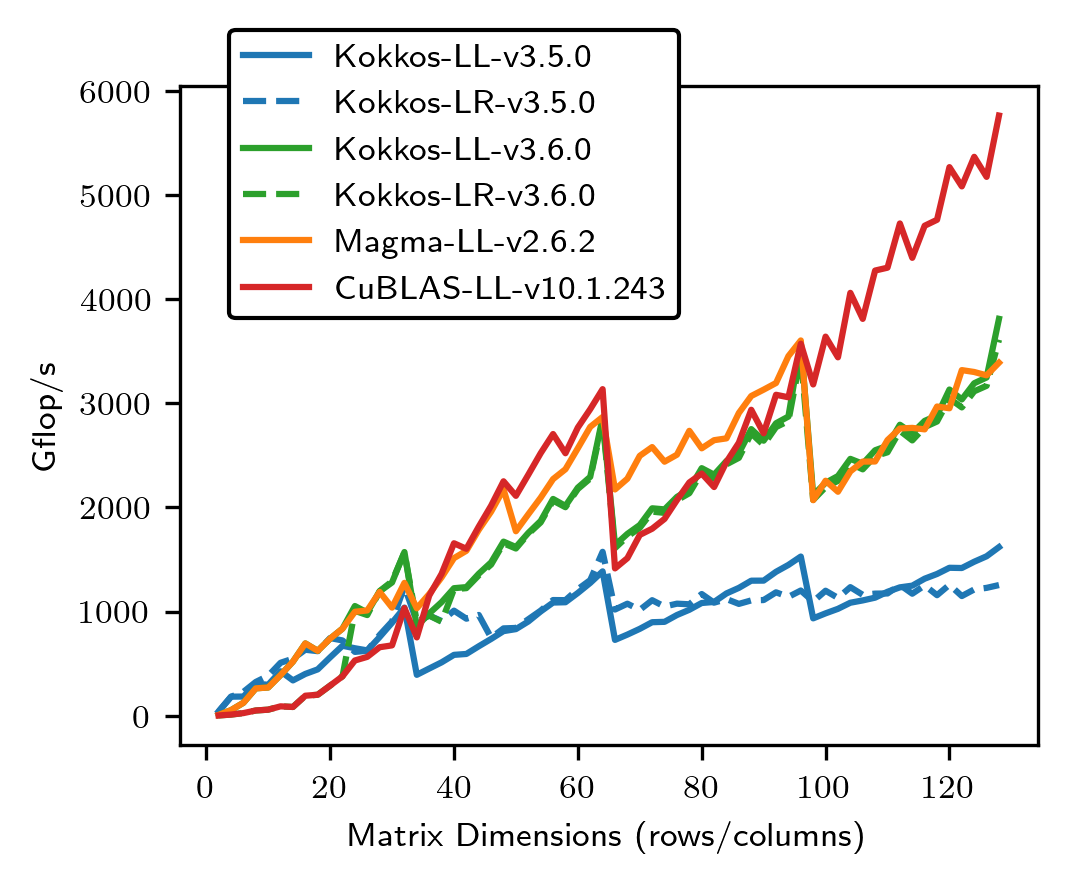
\includegraphics[scale=0.5]{batchedGEMM}
    % \caption{Kokkos BatchedGemm square heuristic, Magma v2.6.2 and CuBlas BatchedGemm on V100 compiled with gcc v8.3.0 and cuda 10.1.243 on V100.}
  \end{figure}
\end{columns}\vspace{1em}
Future work includes additional optimizations to the Kokkos BatchedGemm algorithm.
\end{frame}

\begin{frame}[fragile]{Mixed precision algorithms (Jennifer)}
\begin{columns}[t,onlytextwidth]
  \column{0.475\textwidth}
  \begin{itemize}
  \item Kokkos Kernels provides mixed precisions linear algebra kernels.
  \item GMRES with iterative refinement runs in single precision, residual achieves double precision via iterative refinement
  \item Kokkos Kernels is also providing interfaces for experiments with 16-bit precisions
  \end{itemize}
  \column{0.05\textwidth}
  \column{0.475\textwidth}
  \begin{center}
    \begin{figure}
      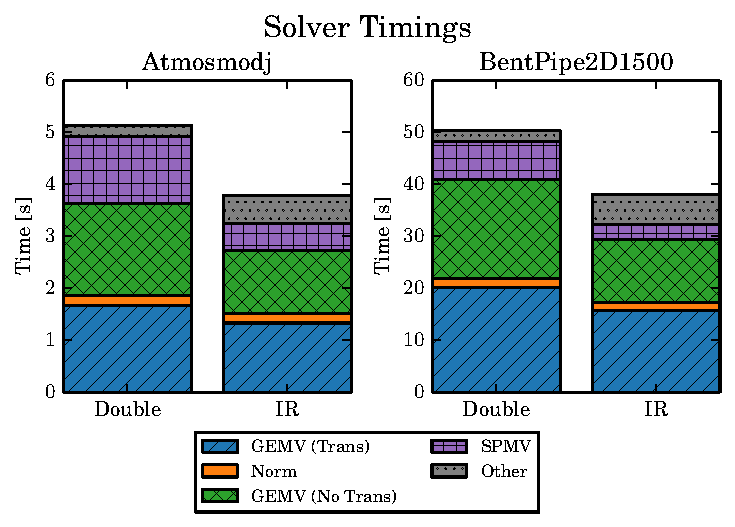
\includegraphics[scale=0.4]{mixed_precision}
      \caption{\tiny Solve times for GMRES(50) double (left) and IR (right) for the matrices Atmosmodj and BentPipe2D1500. Each bar represents total solve time, split up to give a breakdown of time spent in different kernels.}
    \end{figure}
  \end{center}
\end{columns}
\end{frame}

\begin{frame}[fragile]{Collaborations}
Multiple new and ongoing collaborations are cultivated
\begin{itemize}
  \item Nvidia: LU factorization for dense systems
  \item Ginkgo: development of batched gmres
  \item PETSc: providing a portable algebra layer
  \item ExaWind: preconditioner techniques
  \item AMD: library optimization and MFMA usage
  \item ANL: porting and testing on Intel platform
  \item NASA: performance optimization of sparse matrix-vector product
\end{itemize}
and probably many more that I forget...
\end{frame}

\begin{frame}[fragile]{Future focus}
Focus of future work
\begin{itemize}
  \item Performance optimization in Block Sparse algorithms
  \item Format conversion of sparse matrix: Csc2Csr, Coo2Csr
  \item Sparse ILU and TRSV performance improvements
  \item more batched solver features and new batched ODE solvers
  \item more stream support for BLAS and Sparse kernels
  \item fast iterative ILUt algorithm
\end{itemize}
\end{frame}
